\graphicspath{{./}}

\question Suppose you are given this directed, acylic graph below: \\

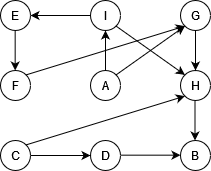
\includegraphics[]{topics/sorting/medium/topological-mechanical/dag.png}

Perform a topological sort on this graph using the DFS postorder method discussed in lecture:
\begin{enumerate}
    \item Find a node with no incoming edge.
    \item Run a DFS post-order traversal from the node with no incoming edge.
    \item While there remain unvisited nodes, start a new DFS post-order traversal from any node with no incoming edge.
    \item A topological sort is the reverse of the order in which the nodes were visited.
\end{enumerate}
Break any ties alphabetically.

\begin{solution}
A DFS post-order search traverses the nodes in the following order:

BHGFEIADC

Meaning our topological search is the reverse of that:

CDAIEFGHB
\end{solution}

\question What is the time complexity of the above algorithm? Give your runtime in terms of $V$, the number of nodes, and $E$, the number of edges.

\begin{solution}
When we start our algorithm, we first iterate through all edges to get the in-degree of each node. This takes $O(E)$ time. To keep track of nodes that have in-degree zero (with respect to nodes that have not been visited), we can maintain a stack of nodes that have in-degree zero.

When we initialize our stack, we take all nodes with in-degree zero and push them onto our stack. This takes $O(V)$ time.

Then, at step 1, we find a node with in-degree zero by popping off the stack. At the end of each DFS traversal, we can get a new node with in-degree 0 in constant time by popping off the stack. Since we visit each edge and vertex at most once, the cost of our DFS searches is therefore $O(E+V)$.

Hence, our overall runtime is $O(E+V)$.
\end{solution}
